%----------------------------------------------------------------------------------------
%    PACKAGES AND THEMES
%----------------------------------------------------------------------------------------

\documentclass[aspectratio=169,xcolor=dvipsnames]{beamer}
\usetheme{SimplePlus}

\usepackage{hyperref}
\usepackage{graphicx} % Allows including images
\usepackage{bbm}
\usepackage{booktabs} % Allows the use of \toprule, \midrule and \bottomrule in table
\hypersetup{
    colorlinks=true, % Enable colored links
    linkcolor=blue, % Color for internal links (e.g., table of contents)
    filecolor=magenta, % Color for file links
    urlcolor=blue, % Color for URLs
    citecolor=green % Color for citations
}

%----------------------------------------------------------------------------------------
%    TITLE PAGE
%----------------------------------------------------------------------------------------

\title{TITLE}

\author{Arturo Abril}

\institute
{
    Vrije Universiteit Amsterdam
}
\date{\today} % Date, can be changed to a custom date

%----------------------------------------------------------------------------------------
%    PRESENTATION SLIDES
%----------------------------------------------------------------------------------------

\begin{document}

\begin{frame}
    % Print the title page as the first slide
    \titlepage
\end{frame}

\begin{frame}{Overview}
    % Throughout your presentation, if you choose to use \section{} and \subsection{} commands, these will automatically be printed on this slide as an overview of your presentation
    \tableofcontents
\end{frame}

%------------------------------------------------
\section{Problem introduction}
%------------------------------------------------

%------------------------------------------------
\begin{frame}
    \huge{...}
\end{frame}
%------------------------------------------------

\begin{frame}{Title}
    Something else
    \vfill
    \begin{itemize}
        \item 1
        \vfill
        \item 2
    \end{itemize}
\end{frame}

\begin{frame}{}
    \begin{figure}
        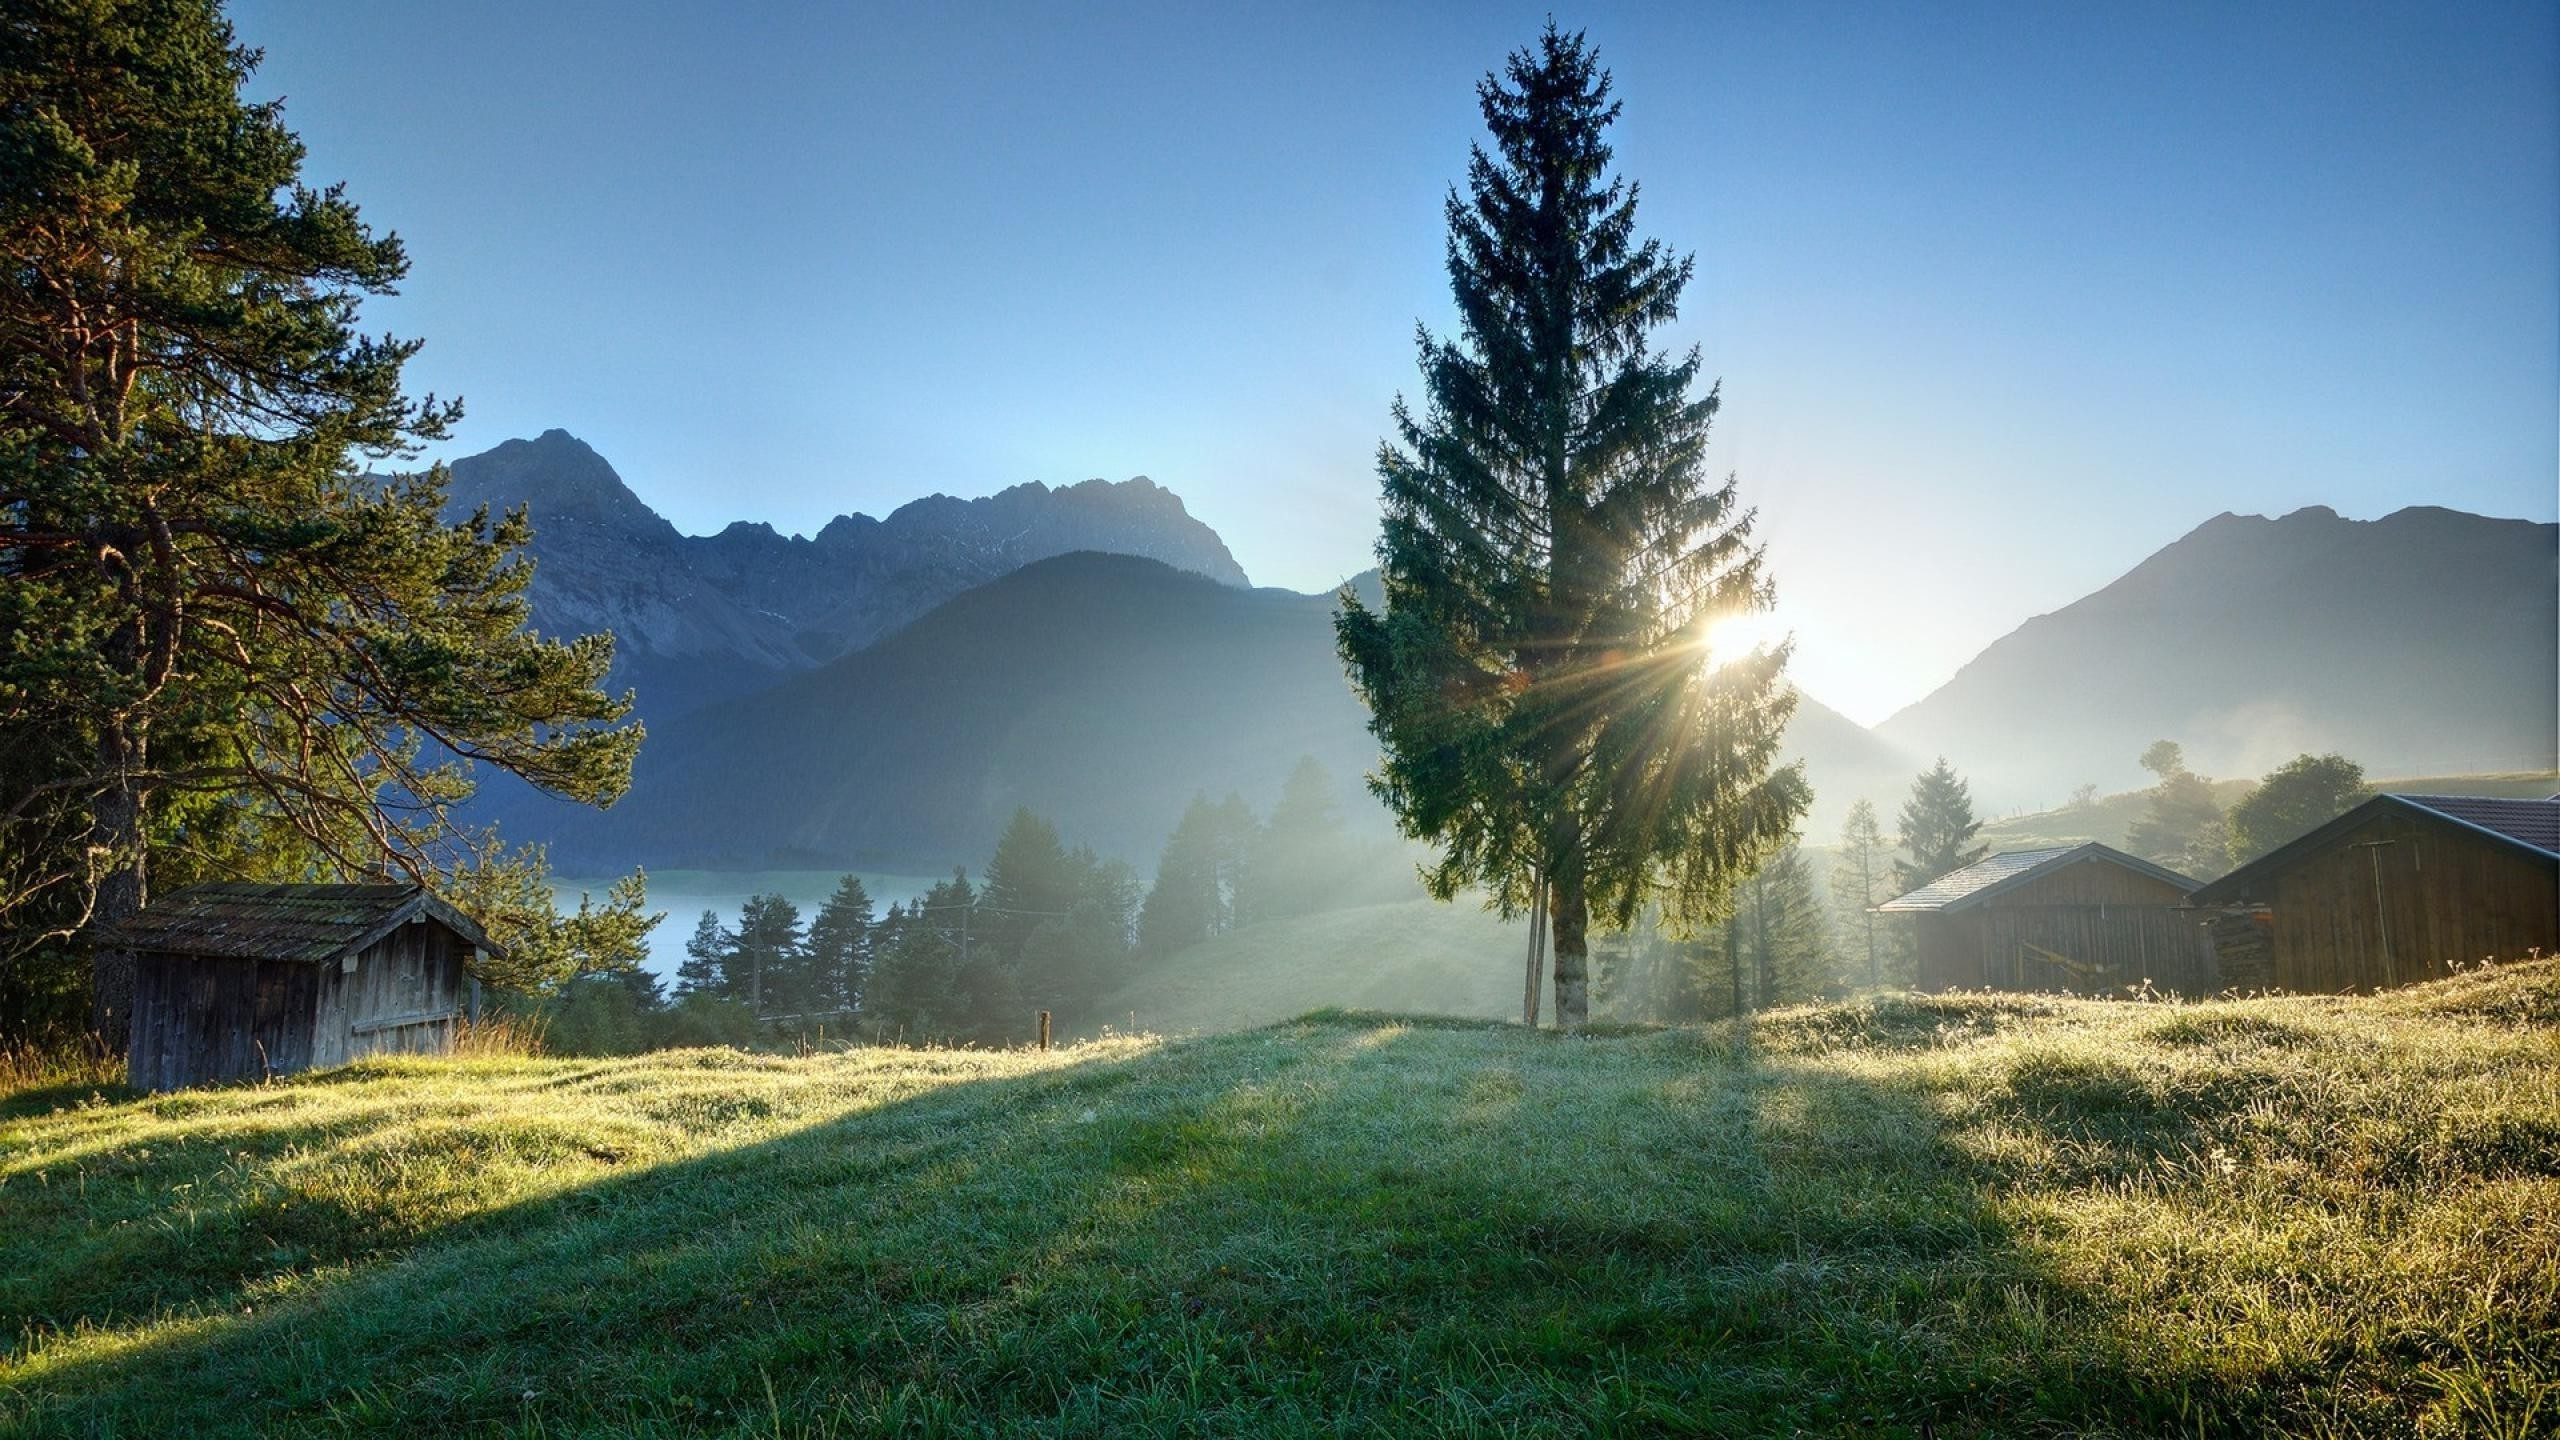
\includegraphics[width=0.8\linewidth]{1.jpg}
    \end{figure}
\end{frame}
%------------------------------------------------

\begin{frame}{Columns}
    Separate slide into columns
    \begin{columns}
        \column{0.5\textwidth}
        \begin{figure}
            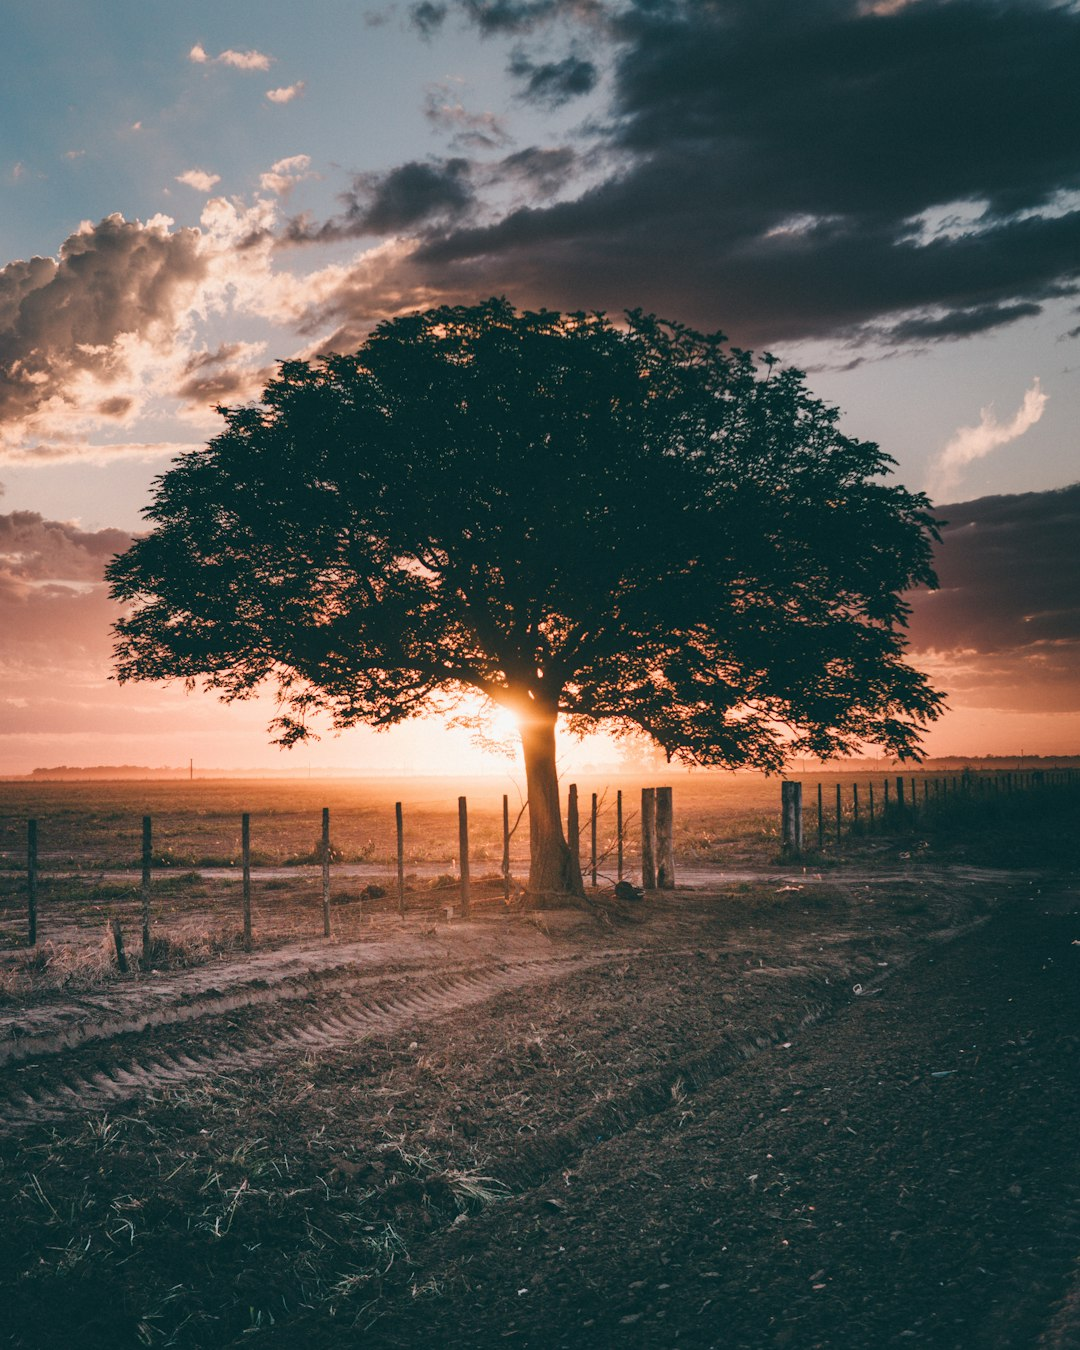
\includegraphics[width=0.5\linewidth]{2.jpg}
        \end{figure}
        \column{0.5\textwidth}
        \begin{figure}
            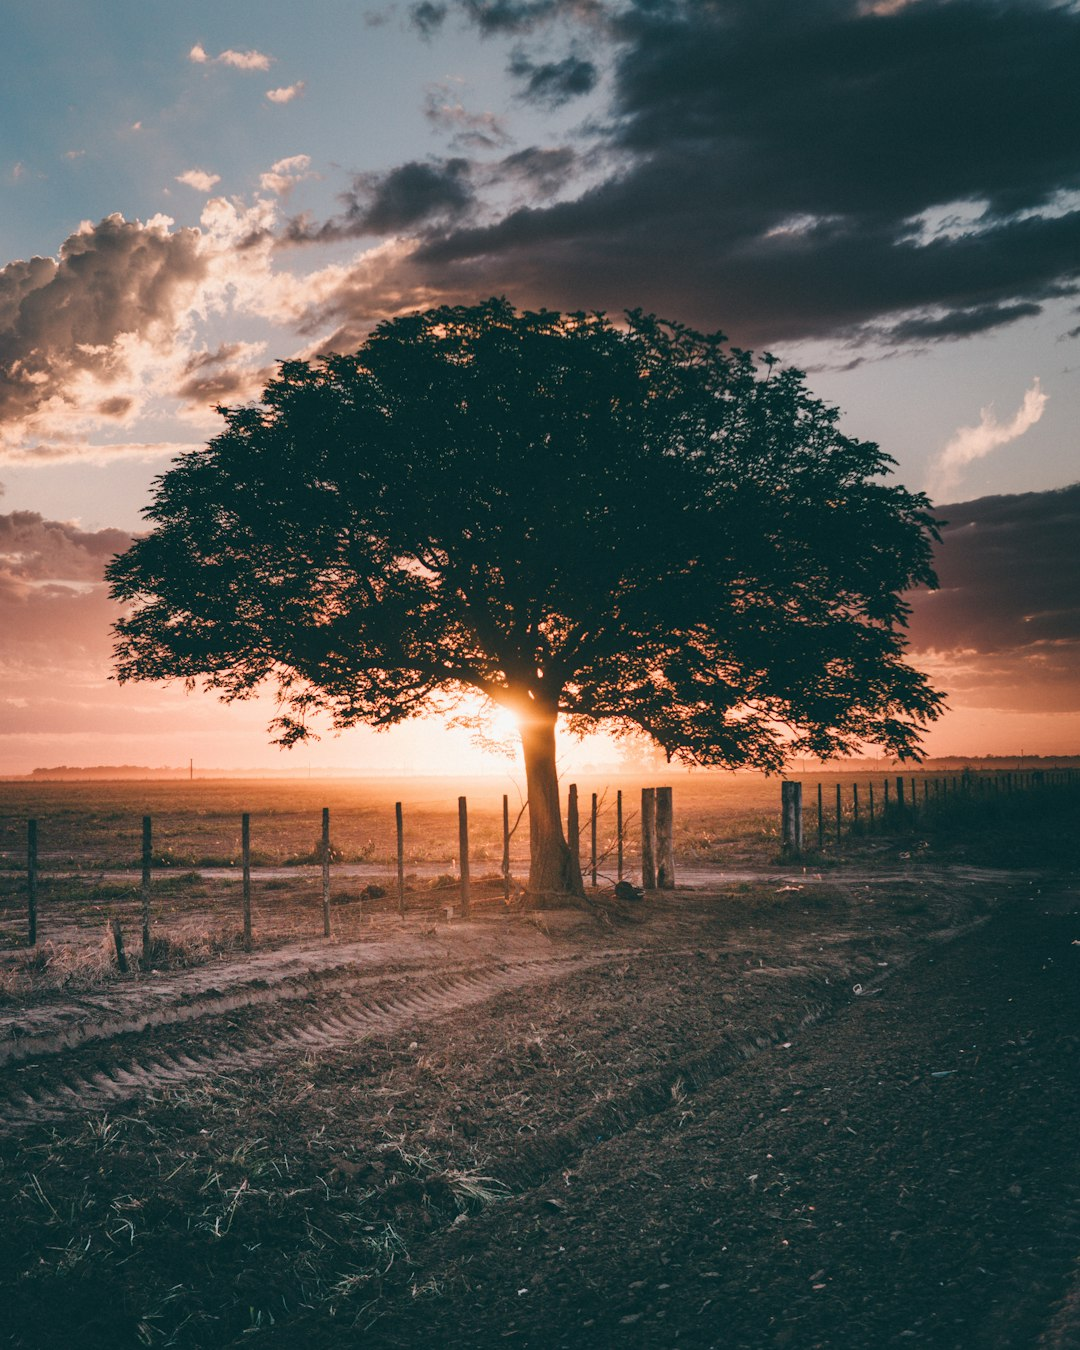
\includegraphics[width=0.5\linewidth]{2.jpg}
        \end{figure}
    \end{columns}
    \end{frame}

%------------------------------------------------

%------------------------------------------------
\section{Other section}
%------------------------------------------------

%------------------------------------------------
\subsection{Subsection}
%------------------------------------------------

%------------------------------------------------
\begin{frame}{More items}
    Even
    \begin{itemize}
        \item 1
        \item 2
        \item 3
    \end{itemize}
\end{frame}
%------------------------------------------------

%------------------------------------------------
\section{Outlook}
%------------------------------------------------

%------------------------------------------------
\begin{frame}{Outlook}
    \begin{itemize}
        \item I did 1
        \item And 2
    \end{itemize}
\end{frame}
%------------------------------------------------



%------------------------------------------------
\begin{frame}
    \Huge{\centerline{\textbf{Thanks}}}
\end{frame}
%------------------------------------------------

%------------------------------------------------
\begin{frame}
    \Huge{\centerline{\textbf{Questions?}}}
\end{frame}
%------------------------------------------------



\end{document}
